\begin{frame}{Observaciones}
  Para un cuadrado $2 \times 2$, puede contener,
  a lo más, $4$ discos unitarios que no se intersecten
  \begin{figure}  
    \centering
    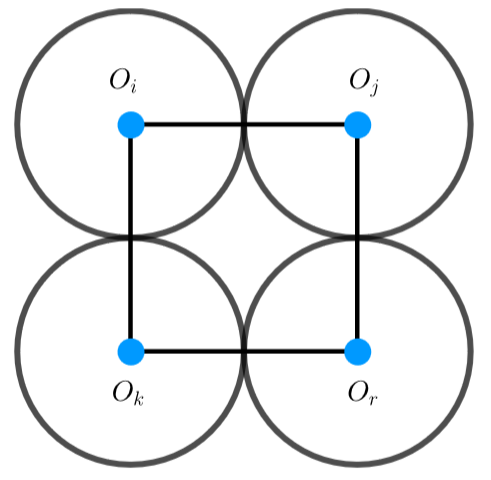
\includegraphics[width=0.4\textwidth]{./Images/4.png}
  \end{figure}
\end{frame}

\begin{frame}{Construcción de rejillas desplazadas}
 Construcción:
  \begin{itemize}[<+->]
  \item Definimos cuadrículas, por conjunto candidato, $G_1, \dotsm, G_k$. Estas pueden
    ser distintas y en ocasiones iguales
    \begin{figure}  
      \centering
      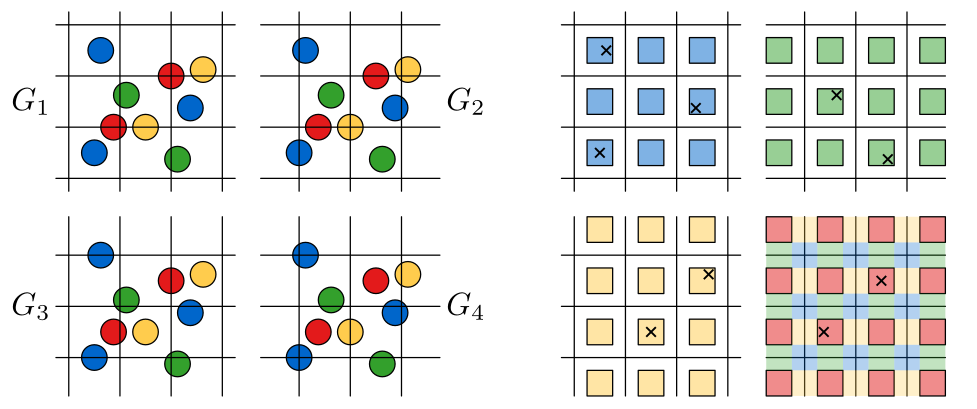
\includegraphics[width=0.4\textwidth]{./Images/cuadricula.png}
    \end{figure}
  \item Cada celda puede ser definida de longitud $4$ o trabajar celdas de
    longitud 2 de manera unificada.
  \item Para $G_1$ tenemos las líneas $\{x = 4i\}$ y $\{y = 4i\}$ con
    $i \in \mathbb{Z}^+$. Análogo para longitud 2.
  \item Para las siguientes $G_2$ y $G_3$ marcamos $\{x = 4i + 2\}$ y $\{y = 4i + 2\}$
    respectivamente.
  \item $G_4$ se deplaza en ambos sentidos $\{x = 4i + 2\}$ y $\{y = 4i + 2\}$. Esto se
    sigue de manera iterativa.
  \item La celda cumple la propiedad de consultar por intersecciones de discos más cercanos
    y enocntrar el disco más lejano dado un disco. La última propiedad no la utilizaremos en
    nuestro caso.
  \end{itemize}
\end{frame}

\begin{frame}
  En nuestro caso, usemos la reja de tamaño $2$, con la concideración de que cada
  centro de disco se encuentra en una única celda. Así, para $S_1$ tenemos que
  \begin{figure}  
    \centering
    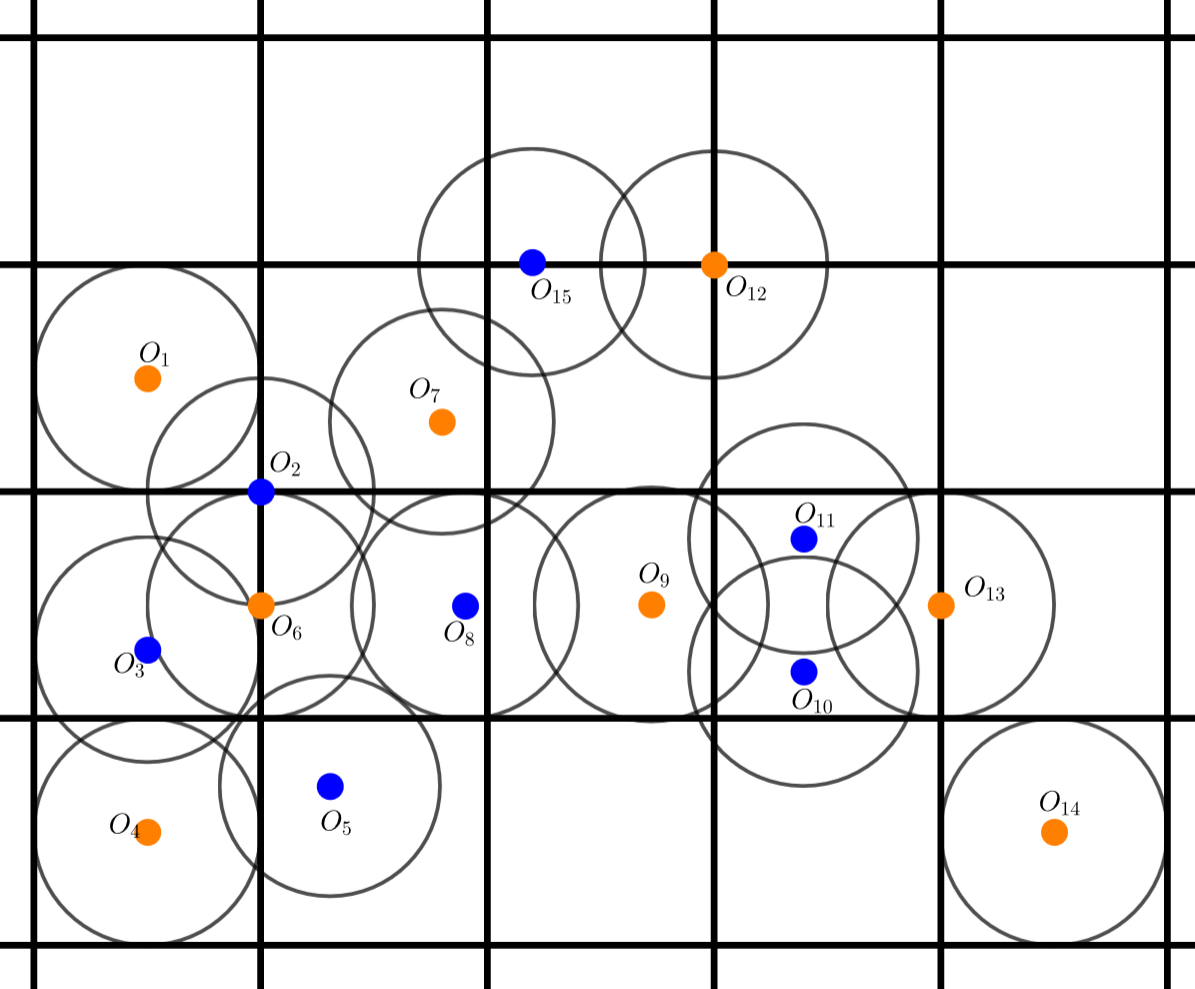
\includegraphics[width=0.7\textwidth]{./Images/R1.png}
  \end{figure}
\end{frame}

\begin{frame}
  Para $S_2$ tenemos que
  \begin{figure}  
    \centering
    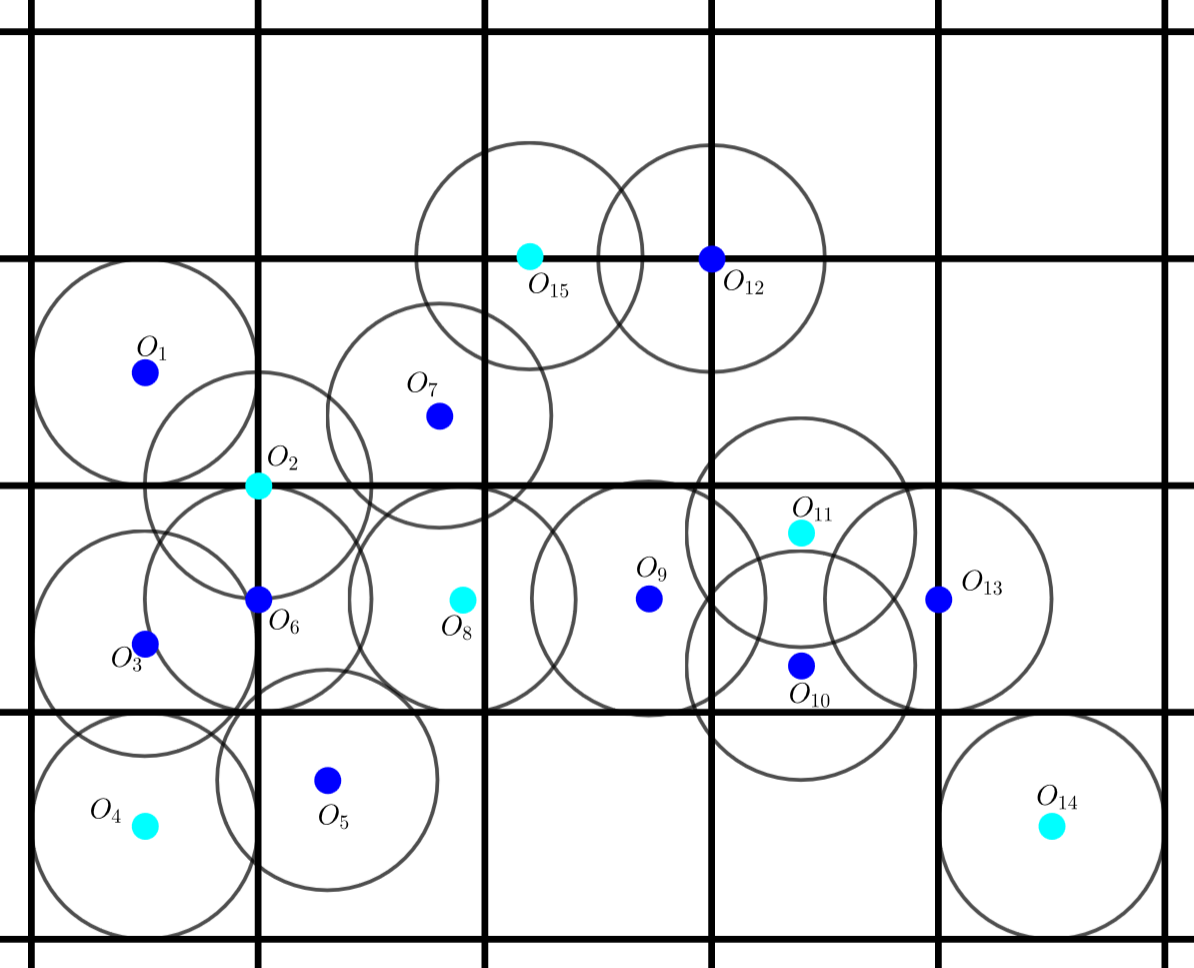
\includegraphics[width=0.7\textwidth]{./Images/R2.png}
  \end{figure}
\end{frame}

\begin{frame}
  Para $S_3$ tenemos que
  \begin{figure}  
    \centering
    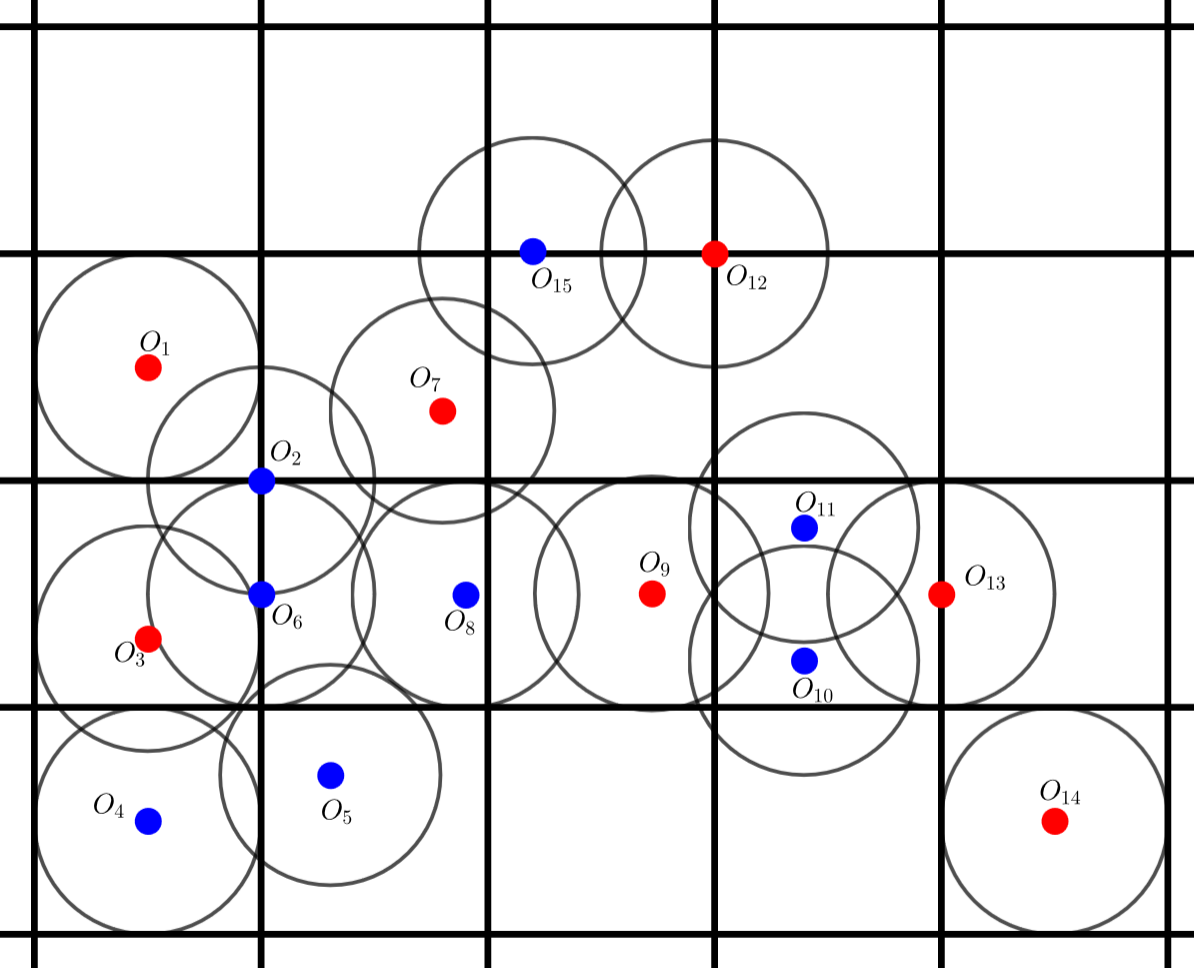
\includegraphics[width=0.7\textwidth]{./Images/R3.png}
  \end{figure}
\end{frame}

\begin{frame}
  \begin{block}{Lema 1.}
    Cada disco unitario en $\mathbb{R}^2$ está contenido en una celda de, al menos, una de las
    cuadrículas desplazadas $G_1, \dotsm, G_k$. En consecuencia para un conjunto $S$ de discos
    unitarios la celda de una de las rejillas contiene conjuntamente
    \[\frac{|S|}{4}\]
    discos.
  \end{block}
  \textbf{Dem.} La primera parte se da a partir de su construcción. La segunda parte se sigue
  del principio de casillas. \hfill $\square$\newline

  Gracias a este lema sabemos que una cuadrícula contiene al menos una fracción constante
  ($o(1)$) de la aproximación de OPT.
\end{frame}


\begin{frame}
  \begin{block}{Lema 2.}
    Sean $S_1, \dotsm S_k$ conjuntos independientes en el conjunto $D$ de discos unitarios
    calculados para $G_1, \dotsm G_k$ respectivamente. El más grande de $S_1, \dotsm,S_k$
    es una $12$-aproximación de MIS, para $D$.
  \end{block}
  \textbf{Dem.} Observar el caso en dónde $|S_i| = 1$ para rejillas $4 \times 4$ (este caso
  no es válido, pero da la idea de la prueba).\newline

  \textbf{Obs.} Una $x$-aproximación es una aproximación en $\frac{1}{x}$ que se puede
  interpretar cómo OPT - $x$, pero núnca cómo OPT + $x$.
\end{frame}
